% ============================================================================
% TOPIC 18A: COLLISION THEORY
% ============================================================================

\section{Topic 18A: Collision Theory}

% ===========================================================================
% Slide 6: Topic 18A Overview
% ===========================================================================
\begin{frame}{Topic 18A: Collision Theory}

\begin{columns}[T]

\column{0.5\textwidth}
\textbf{The Simplest Model:}

\vspace{0.2cm}

Reactions occur when molecules collide \textit{if}:

\begin{enumerate}
\item They collide with sufficient frequency
\item They have enough kinetic energy ($\ge E_a$)
\item They have correct orientation (steric factor)
\end{enumerate}

\vspace{0.2cm}

\textbf{Learning Objectives:}
\begin{itemize}
\item Derive collision rate from kinetic theory
\item Connect to Arrhenius equation
\item Understand steric factors
\item Apply to unimolecular reactions
\end{itemize}

\column{0.5\textwidth}
\centering

\begin{tikzpicture}[scale=0.65]
% Successful collision
\node[font=\small] at (0,3.5) {\textbf{Successful Collision}};
\draw[-{Stealth[length=3mm]},thick,red] (-2,3) -- (-0.5,3);
\node[circle,draw,fill=blue!30,minimum size=0.8cm] at (-2,3) {A};
\node[circle,draw,fill=red!30,minimum size=0.8cm] at (0,3) {B};
\draw[-{Stealth[length=3mm]},thick,green!70!black] (0.5,3) -- (2,3);
\node[circle,draw,fill=green!30,minimum size=0.8cm] at (2,3) {P};
\node[font=\tiny,text=green!70!black] at (1.2,2.5) {$E \ge E_a$, correct angle};

% Failed collision - not enough energy
\node[font=\small] at (0,1.5) {\textbf{Failed: Low Energy}};
\draw[-{Stealth[length=3mm]},thick,red] (-2,1) -- (-0.5,1);
\node[circle,draw,fill=blue!30,minimum size=0.8cm] at (-2,1) {A};
\node[circle,draw,fill=red!30,minimum size=0.8cm] at (0,1) {B};
\draw[-{Stealth[length=3mm]},thick,gray,dashed] (0.5,1) -- (2,1);
\node[circle,draw,fill=blue!30,minimum size=0.8cm] at (1.5,1) {A};
\node[circle,draw,fill=red!30,minimum size=0.8cm] at (2,1) {B};
\node[font=\tiny,text=gray] at (1.2,0.5) {$E < E_a$: bounce};

% Failed collision - wrong orientation
\node[font=\small] at (0,-0.5) {\textbf{Failed: Wrong Orientation}};
\draw[-{Stealth[length=3mm]},thick,red] (-2,-1) -- (-0.3,-1);
\node[circle,draw,fill=blue!30,minimum size=0.8cm] at (-2,-1) {A};
\node[circle,draw,fill=red!30,minimum size=0.8cm] at (0,-1.2) {B};
\draw[-{Stealth[length=3mm]},thick,gray,dashed] (0.3,-1) -- (1.5,-0.5);
\draw[-{Stealth[length=3mm]},thick,gray,dashed] (0.3,-1.2) -- (1.5,-1.7);
\node[font=\tiny,text=gray] at (1,-1.7) {Glancing: $P < 1$};
\end{tikzpicture}

\end{columns}

\end{frame}

% ===========================================================================
% Slide: Kinetic Molecular Theory Background
% ===========================================================================
\begin{frame}{Kinetic Molecular Theory Background}

\textbf{Maxwell-Boltzmann Distribution of Speeds:}

The fraction of molecules with speeds between $v$ and $v + dv$:

\[ f(v) = 4\pi \left(\frac{m}{2\pi \kB T}\right)^{3/2} v^2 e^{-mv^2/2\kB T} \]

\begin{columns}[T]
\column{0.5\textwidth}
\textbf{Key Quantities:}
\begin{itemize}
\item Mean speed: $\bar{v} = \left(\frac{8\kB T}{\pi m}\right)^{1/2}$
\item Root-mean-square: $v_{rms} = \left(\frac{3\kB T}{m}\right)^{1/2}$
\item Most probable: $v_p = \left(\frac{2\kB T}{m}\right)^{1/2}$
\end{itemize}

\column{0.5\textwidth}
\centering
\includegraphics[width=\textwidth]{Reaction_Dynamics_Interactive/images/maxwell_boltzmann_speeds.png}

\vspace{0.2cm}
\tiny \textit{Interactive version: Scan QR code at end of topic}
\end{columns}

\end{frame}

% ===========================================================================
% Slide: Collision Cross-Section - Detailed
% ===========================================================================
\begin{frame}{Collision Cross-Section - Hard Sphere Model}

\begin{columns}[T]
\column{0.5\textwidth}
\textbf{Geometric Definition:}
\begin{itemize}
\item Treat molecules as hard spheres
\item Radii $r_A$ and $r_B$
\item Collision occurs when centers approach within $d = r_A + r_B$
\item Target area: $\sigma = \pi d^2$
\end{itemize}

\vspace{0.2cm}
\keyeq{\sigma = \pi d^2 = \pi (r_A + r_B)^2}

\textbf{Impact Parameter $b$:}
\begin{itemize}
\item Perpendicular distance between trajectories
\item Collision if $b \le d$
\end{itemize}

\column{0.5\textwidth}
\centering
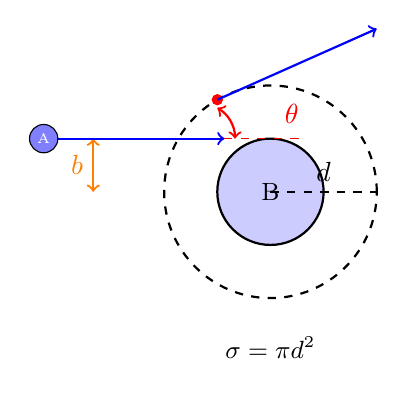
\begin{tikzpicture}[scale=0.9]
    % Target molecule (center)
    \draw[fill=blue!20, thick] (0,0) circle (0.75cm);
    \node at (0,0) {\small B};

    % Collision diameter
    \draw[dashed, thick] (0,0) circle (1.5cm);
    \draw[dashed, thick] (0,0) -- (1.5,0) node[midway, above] {$d$};

    % Impact parameter b = 0.75 cm
    \draw[red, dashed] (-3, 0.75) -- (0.5, 0.75);
    \draw[<->, orange, thick] (-2.5, 0) -- (-2.5, 0.75) node[midway, left] {$b$};

    % Projectile molecule A trajectory
    % Incoming straight line
    \draw[->, thick, blue] (-3.2, 0.75) -- (-0.65, 0.75);
    \draw[fill=blue!50] (-3.2, 0.75) circle (0.2cm) node[white] {\tiny A};

    % Contact point at angle θ from center
    \coordinate (contact) at ({-1.5*0.5},{1.5*0.866}); % at 120 degrees
    \fill[red] (contact) circle (0.08cm);

    % Outgoing deflected trajectory
    \draw[->, thick, blue] (contact) -- (1.5, 2.3);

    % Scattering angle
    \draw[<->, red, thick] (-0.5, 0.75) arc[start angle=0, end angle=60, radius=0.5cm];
    \node[red] at (0.3, 1.1) {$\theta$};

    % Label
    \node at (0,-2.2) {\small $\sigma = \pi d^2$};
\end{tikzpicture}
\end{columns}

\vspace{0.2cm}
\textbf{Typical Values:} $d \approx 0.3-0.5$ nm, $\sigma \approx 0.1-1$ nm$^2$ (10-100 \AA$^2$)

\end{frame}

% ===========================================================================
% Slide: Derivation of Collision Rate - Part 1
% ===========================================================================
\begin{frame}{Derivation of Collision Rate (Part 1)}

\textbf{Setup:} Consider molecule A moving through gas of B molecules.

\vspace{0.3cm}

\textbf{Step 1: Collision Cylinder}
\begin{itemize}
\item In time $\Delta t$, A sweeps volume $V = \sigma v_{rel} \Delta t$
\item Number of B molecules in cylinder: $N_B = \mathcal{N}_B \cdot \sigma v_{rel} \Delta t$
\item Collision rate for one A: $\sigma v_{rel} \mathcal{N}_B$
\end{itemize}

\vspace{0.3cm}

\textbf{Step 2: Average Over Velocity Distribution}
\begin{itemize}
\item Must average over Maxwell-Boltzmann distribution of $v_{rel}$
\item For two species: $\bar{v}_{rel} = \left(\frac{8\kB T}{\pi \mu}\right)^{1/2}$
\item Reduced mass: $\mu = \frac{m_A m_B}{m_A + m_B}$
\end{itemize}

\end{frame}

% ===========================================================================
% Slide: Derivation of Collision Rate - Part 2
% ===========================================================================
\begin{frame}{Derivation of Collision Rate (Part 2)}

\textbf{Step 3: Total Collision Density}

Total collisions per unit volume per unit time between A and B molecules:

\vspace{0.5cm}

\keyeq{Z_{AB} = \sigma \left(\frac{8\kB T}{\pi \mu}\right)^{1/2} \mathcal{N}_A \mathcal{N}_B}

\vspace{0.5cm}

\textbf{Physical Interpretation:}
\begin{itemize}
\item $\sigma$ = collision cross-section (geometric factor)
\item $\bar{v}_{rel} = \left(\frac{8\kB T}{\pi \mu}\right)^{1/2}$ = mean relative speed
\item $\mathcal{N}_A$, $\mathcal{N}_B$ = number densities (molecules per unit volume)
\item $Z_{AB}$ has units: collisions m$^{-3}$ s$^{-1}$
\end{itemize}

\end{frame}

% ===========================================================================
% Slide: Collision Rate - Identical Molecules
% ===========================================================================
\begin{frame}{Special Case: Identical Molecules}

For collisions between identical molecules A + A:

\vspace{0.2cm}

\textbf{Modified Formula:}
\begin{itemize}
\item Must avoid double-counting (each collision counted twice)
\item Factor of $1/2$ correction
\end{itemize}

\keyeq{Z_{AA} = \frac{1}{2} \sigma \left(\frac{8\kB T}{\pi \mu}\right)^{1/2} \mathcal{N}_A^2}

\vspace{0.2cm}

\textbf{For identical molecules:}
\begin{itemize}
\item $\mu = m_A/2$ (reduced mass)
\item $\bar{v}_{rel} = \sqrt{2} \bar{v}$ where $\bar{v}$ is mean speed of one molecule
\item Collision frequency is $\sqrt{2}$ times what you'd naively expect
\end{itemize}

\end{frame}

% ===========================================================================
% Slide: Worked Example - Collision Density Part 1
% ===========================================================================
\begin{frame}{Worked Example: Collision Rate for N$_2$ (Part 1)}

\textbf{Problem:} Calculate $Z_{N_2-N_2}$ for nitrogen gas at 298 K and 1 bar.
Given: $\sigma \approx 0.43$ nm$^2$ = $4.3 \times 10^{-19}$ m$^2$

\vspace{0.3cm}

\textbf{Step 1: Number density from ideal gas law}
\[ \mathcal{N} = \frac{P}{\kB T} = \frac{10^5 \text{ Pa}}{(1.381 \times 10^{-23} \text{ J K}^{-1})(298 \text{ K})} = 2.43 \times 10^{25} \text{ m}^{-3} \]

\vspace{0.3cm}

\textbf{Step 2: Mean relative speed}

Mass of N$_2$: $m = 28$ amu $= 4.65 \times 10^{-26}$ kg

Reduced mass: $\mu = m/2 = 2.32 \times 10^{-26}$ kg

\[ \bar{v}_{rel} = \sqrt{\frac{8 \times 1.381 \times 10^{-23} \times 298}{\pi \times 2.32 \times 10^{-26}}} = 670 \text{ m s}^{-1} \]

\end{frame}

% ===========================================================================
% Slide: Worked Example - Collision Density Part 2
% ===========================================================================
\begin{frame}{Worked Example: Collision Rate for N$_2$ (Part 2)}

\textbf{Step 3: Calculate collision density}

Using the formula: $Z_{N_2-N_2} = \frac{1}{2} \sigma \bar{v}_{rel} \mathcal{N}^2$

\vspace{0.3cm}

\[ Z_{N_2-N_2} = \frac{1}{2} \times 4.3 \times 10^{-19} \times 670 \times (2.43 \times 10^{25})^2 \]

\vspace{0.3cm}

\[ \boxed{Z_{N_2-N_2} \approx 5 \times 10^{34} \text{ collisions m}^{-3} \text{ s}^{-1}} \]

\vspace{0.3cm}

\textbf{Interpretation:} This enormous collision rate shows why most gas reactions require activation energy - if every collision reacted, all reactions would be instantaneous!

\end{frame}

% ===========================================================================
% Slide: Energy Requirements - Boltzmann Factor
% ===========================================================================
\begin{frame}{Energy Requirements: Not All Collisions React}

\textbf{The Problem:}
\begin{itemize}
\item $Z_{AB} \sim 10^{34}$ collisions m$^{-3}$ s$^{-1}$ is enormous!
\item If every collision led to reaction, all reactions would be over in nanoseconds
\item Reality: Most reactions have measurable rates (seconds to hours)
\end{itemize}

\vspace{0.3cm}

\textbf{The Solution: Activation Energy}
\begin{itemize}
\item Only collisions with kinetic energy $\varepsilon \ge E_a$ along line of centers react
\item Fraction of molecules with energy $> E_a$ from Boltzmann distribution:
\end{itemize}

\keyeq{f(E > E_a) = \int_{E_a}^{\infty} f(E) dE = e^{-E_a/RT}}

\vspace{0.2cm}
\emphbox{The exponential factor dramatically reduces the reactive collision rate}

\end{frame}

% ===========================================================================
% Slide: Energy Distribution
% ===========================================================================
\begin{frame}{Maxwell-Boltzmann Energy Distribution}

The fraction of molecules with translational energy between $\varepsilon$ and $\varepsilon + d\varepsilon$:

\[ f(\varepsilon) = \frac{2\pi}{(\pi \kB T)^{3/2}} \varepsilon^{1/2} e^{-\varepsilon/\kB T} \]

\begin{columns}[T]
\column{0.5\textwidth}
\textbf{Key Features:}
\begin{itemize}
\item Maximum at $\varepsilon = \kB T/2$
\item Mean energy: $\langle \varepsilon \rangle = \frac{3}{2}\kB T$
\item High-energy tail decays exponentially
\item Fraction with $\varepsilon > E_a$: \[\int_{E_a}^{\infty} f(\varepsilon) d\varepsilon = e^{-E_a/\kB T}\]
\end{itemize}

\column{0.5\textwidth}
\centering
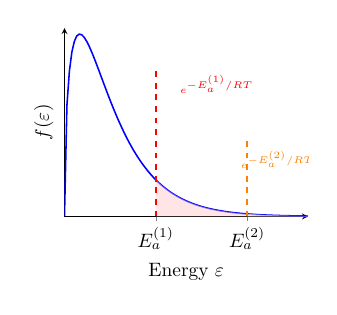
\begin{tikzpicture}[scale=0.7]
\begin{axis}[
    xlabel={Energy $\varepsilon$},
    ylabel={$f(\varepsilon)$},
    axis lines=left,
    xmin=0, xmax=8,
    ymin=0, ymax=0.5,
    xtick={3,6},
    xticklabels={$E_a^{(1)}$, $E_a^{(2)}$},
    ytick=\empty,
    width=6cm,
    height=5cm
]
% Correct Maxwell-Boltzmann energy distribution: f(ε) = (2/√π)√ε exp(-ε)
\addplot[blue, thick, domain=0:8, samples=100] {2/sqrt(pi)*sqrt(x)*exp(-x)};
\addplot[fill=red!20, draw=none, opacity=0.5, domain=3:8, samples=50] {2/sqrt(pi)*sqrt(x)*exp(-x)} \closedcycle;
\addplot[fill=orange!20, draw=none, opacity=0.5, domain=6:8, samples=30] {2/sqrt(pi)*sqrt(x)*exp(-x)} \closedcycle;
\draw[red, dashed, thick] (axis cs:3,0) -- (axis cs:3,0.4);
\draw[orange, dashed, thick] (axis cs:6,0) -- (axis cs:6,0.2);
\node[red] at (axis cs:5,0.35) {\tiny $e^{-E_a^{(1)}/RT}$};
\node[orange] at (axis cs:7,0.15) {\tiny $e^{-E_a^{(2)}/RT}$};
\end{axis}
\end{tikzpicture}
\end{columns}

\textbf{Higher $E_a$ $\Rightarrow$ Smaller reactive fraction $\Rightarrow$ Slower reaction}

\end{frame}

% ===========================================================================
% Slide: Energy-Dependent Cross-Section
% ===========================================================================
\begin{frame}{Reactive Cross-Section: Energy Dependence}

The collision cross-section depends on collision energy $\varepsilon$:

\keyeq{\sigma_r(\varepsilon) = \begin{cases}
0 & \varepsilon < E_a \\
\sigma \left(1 - \frac{E_a}{\varepsilon}\right) & \varepsilon \ge E_a
\end{cases}}

\begin{columns}[T]
\column{0.55\textwidth}
\textbf{Physical Interpretation:}
\begin{itemize}
\item Below $E_a$: No reaction possible ($\sigma_r = 0$)
\item At $E_a$: Reaction just becomes possible ($\sigma_r = 0$)
\item Well above $E_a$: Approaches geometric $\sigma$
\item The factor $(1 - E_a/\varepsilon)$ represents the "likelihood" of having enough energy in the right direction
\end{itemize}

\column{0.45\textwidth}
\centering
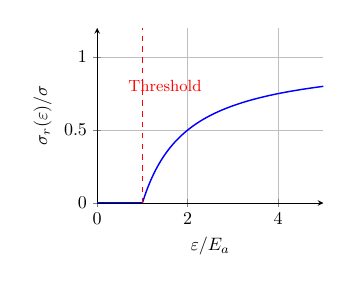
\begin{tikzpicture}[scale=0.65]
\begin{axis}[
    xlabel={$\varepsilon/E_a$},
    ylabel={$\sigma_r(\varepsilon)/\sigma$},
    xmin=0, xmax=5,
    ymin=0, ymax=1.2,
    axis lines=left,
    grid=major,
    width=6cm,
    height=5cm
]
\addplot[blue, thick, domain=1:5, samples=100] {1 - 1/x};
\addplot[blue, thick, domain=0:1, samples=2] {0};
\draw[red, dashed] (axis cs:1,0) -- (axis cs:1,1.2);
\node[red] at (axis cs:1.5,0.8) {\small Threshold};
\end{axis}
\end{tikzpicture}

\vspace{0.2cm}
\small The linear rise from threshold is a simplified model; real reactions may have different energy dependencies.
\end{columns}

\end{frame}

% ===========================================================================
% Slide: Derivation of Rate Constant
% ===========================================================================
\begin{frame}{Derivation of the Collision Theory Rate Constant}

\textbf{Starting Point:} Reactive collision rate per unit volume

\[ \text{Rate} = \int_0^{\infty} \sigma_r(\varepsilon) v_{rel}(\varepsilon) \mathcal{N}_A \mathcal{N}_B f(\varepsilon) d\varepsilon \]

\textbf{Key Steps:}
\begin{enumerate}
\item Insert $\sigma_r(\varepsilon) = \sigma(1 - E_a/\varepsilon)$ for $\varepsilon \ge E_a$
\item Use $v_{rel} = \sqrt{2\varepsilon/\mu}$ (relation between speed and energy)
\item Integrate over Boltzmann distribution $f(\varepsilon) \propto e^{-\varepsilon/\kB T}$
\end{enumerate}

\vspace{0.2cm}

\textbf{Result after integration:}

\keyeq{k_r = \NA \sigma \left(\frac{8\kB T}{\pi \mu}\right)^{1/2} e^{-E_a/RT}}

\vspace{0.2cm}

\textbf{In terms of molar concentrations $[A]$, $[B]$:}
\[ \text{Rate} = k_r [A][B] \]

\end{frame}

% ===========================================================================
% Slide: Connection to Arrhenius Equation
% ===========================================================================
\begin{frame}{Connection to Arrhenius Equation}

\textbf{Collision Theory Result:}
\[ k_r = \NA \sigma \left(\frac{8\kB T}{\pi \mu}\right)^{1/2} e^{-E_a/RT} \]

\textbf{Arrhenius Empirical Form:}
\[ k = A e^{-E_a/RT} \]

\vspace{0.3cm}

\textbf{Identification of Pre-exponential Factor:}
\keyeq{A_{theory} = \NA \sigma \left(\frac{8\kB T}{\pi \mu}\right)^{1/2}}

\begin{itemize}
\item Typical values: $A \sim 10^{10} - 10^{11}$ dm$^3$ mol$^{-1}$ s$^{-1}$ for bimolecular gas reactions
\item Temperature dependence: $A \propto T^{1/2}$ (weak, often ignored)
\item For Arrhenius plots ($\ln k$ vs $1/T$): slope = $-E_a/R$, intercept = $\ln A$
\end{itemize}

\end{frame}

% ===========================================================================
% Slide: Numerical Example of A-factor Part 1
% ===========================================================================
\begin{frame}{Numerical Calculation of $A$-factor (Part 1)}

\textbf{Example:} Calculate $A$ for H$_2$ + I$_2 \to$ 2HI at 600 K

\vspace{0.2cm}

\textbf{Given:}
\begin{itemize}
\item $\sigma = 0.30$ nm$^2$ = $3.0 \times 10^{-19}$ m$^2$
\item $m_{H_2} = 2.016$ amu = $3.35 \times 10^{-27}$ kg
\item $m_{I_2} = 253.8$ amu = $4.22 \times 10^{-25}$ kg
\end{itemize}

\vspace{0.3cm}

\textbf{Step 1: Reduced mass}
\[ \mu = \frac{m_{H_2} \cdot m_{I_2}}{m_{H_2} + m_{I_2}} = \frac{3.35 \times 10^{-27} \times 4.22 \times 10^{-25}}{4.25 \times 10^{-25}} = 3.32 \times 10^{-27} \text{ kg} \]

\vspace{0.3cm}

\textbf{Step 2: Mean relative speed}
\[ \bar{v}_{rel} = \sqrt{\frac{8 \times 1.381 \times 10^{-23} \times 600}{3.14159 \times 3.32 \times 10^{-27}}} = 2520 \text{ m s}^{-1} \]

\end{frame}

% ===========================================================================
% Slide: Numerical Example of A-factor Part 2
% ===========================================================================
\begin{frame}{Numerical Calculation of $A$-factor (Part 2)}

\textbf{Step 3: Calculate A-factor}

Using the formula: $A = \NA \sigma \bar{v}_{rel}$

\vspace{0.2cm}

\[ A = 6.022 \times 10^{23} \times 3.0 \times 10^{-19} \times 2520 \]

\[ A = 4.6 \times 10^8 \text{ m}^3 \text{ mol}^{-1} \text{ s}^{-1} \]

\vspace{0.2cm}

Converting to dm$^3$ (multiply by $10^3$):

\[ \boxed{A = 4.6 \times 10^{11} \text{ dm}^3 \text{ mol}^{-1} \text{ s}^{-1}} \]

\vspace{0.15cm}

\textbf{Interpretation:} This is in the typical range $10^{10}-10^{11}$ for bimolecular gas reactions, consistent with collision theory predictions!

\end{frame}

% ===========================================================================
% Slide: The Steric Factor Problem
% ===========================================================================
\begin{frame}{The Steric Factor Problem}

\textbf{Experiment vs Theory:} Does $A_{exp}$ match $A_{theory}$?

\vspace{0.2cm}

\begin{table}
\centering
\small
\begin{tabular}{lccc}
\toprule
\textbf{Reaction} & $\mathbf{A_{exp}}$ & $\mathbf{A_{theory}}$ & $\mathbf{P = A_{exp}/A_{theory}}$ \\
 & (dm$^3$ mol$^{-1}$ s$^{-1}$) & (dm$^3$ mol$^{-1}$ s$^{-1}$) & \\
\midrule
2NOCl $\to$ 2NO + Cl$_2$ & $9.4 \times 10^9$ & $5.9 \times 10^{10}$ & 0.16 \\
2ClO $\to$ Cl$_2$ + O$_2$ & $6.3 \times 10^7$ & $2.5 \times 10^{10}$ & 0.0025 \\
H$_2$ + C$_2$H$_4 \to$ C$_2$H$_6$ & $1.2 \times 10^6$ & $7.3 \times 10^{10}$ & $1.7 \times 10^{-5}$ \\
K + Br$_2 \to$ KBr + Br & $1.0 \times 10^{12}$ & $2.1 \times 10^{11}$ & \alert{4.8} \\
\bottomrule
\end{tabular}
\end{table}

\vspace{0.3cm}

\textbf{Observations:}
\begin{itemize}
\item \textbf{Usually $P < 1$:} Not all orientations are reactive (steric hindrance)
\item \textbf{Complex molecules:} Smaller $P$ (need precise alignment)
\item \textbf{Sometimes $P > 1$:} Long-range forces extend reactive range (Harpoon mechanism)
\end{itemize}

\end{frame}

% ===========================================================================
% Slide: Steric Factor - Physical Basis Part 1
% ===========================================================================
\begin{frame}{The Steric Factor: Modified Collision Theory}

\textbf{Modified Collision Theory:}

\keyeq{k_r = P \cdot \NA \sigma \left(\frac{8\kB T}{\pi \mu}\right)^{1/2} e^{-E_a/RT}}

\vspace{0.15cm}

\textbf{What is P?}
\begin{itemize}
\item \textbf{Steric factor:} Fraction of collisions with proper orientation
\item Effective reactive cross-section: $\sigma_r = P \sigma$
\item Depends on molecular geometry and reaction mechanism
\item Accounts for orientation requirements
\end{itemize}

\vspace{0.15cm}

\textbf{Examples:}
\begin{itemize}
\item \textbf{Atoms:} $P \approx 1$ (spherically symmetric)
\item \textbf{Linear molecules:} $P \sim 0.1-1$ (need end-on approach)
\item \textbf{Complex molecules:} $P \sim 10^{-6}-10^{-2}$ (specific reactive site)
\end{itemize}

\end{frame}

% ===========================================================================
% Slide: Steric Factor - Reactive Geometry
% ===========================================================================
\begin{frame}{The Steric Factor: Reactive Geometry}

\begin{columns}[T]
\column{0.5\textwidth}
\textbf{Orientation Matters:}

\vspace{0.1cm}

Only certain collision geometries lead to reaction:
\begin{itemize}
\item \textcolor{green!70!black}{\textbf{Reactive:}} Attack at reactive site
\item \textcolor{red}{\textbf{Non-reactive:}} Wrong orientation or glancing collision
\end{itemize}

\vspace{0.15cm}

The steric factor $P$ quantifies the fraction of properly oriented collisions.

\column{0.5\textwidth}
\centering
\textbf{Reactive Geometry:}

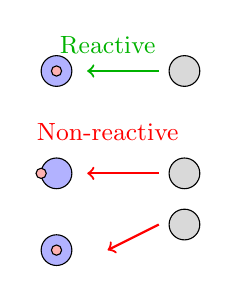
\begin{tikzpicture}[scale=0.65]
% Reactive approach
\node at (0,2.5) {\small \textcolor{green!70!black}{Reactive}};
\draw[fill=blue!30] (-1,2) circle (0.3cm);
\draw[fill=red!30] (-1,2) circle (0.1cm);
\draw[->, thick, green!70!black] (1,2) -- (-0.4,2);
\draw[fill=gray!30] (1.5,2) circle (0.3cm);

% Non-reactive approach 1
\node at (0,0.8) {\small \textcolor{red}{Non-reactive}};
\draw[fill=blue!30] (-1,0) circle (0.3cm);
\draw[fill=red!30] (-1.3,0) circle (0.1cm);
\draw[->, thick, red] (1,0) -- (-0.4,0);
\draw[fill=gray!30] (1.5,0) circle (0.3cm);

% Non-reactive approach 2
\draw[fill=blue!30] (-1,-1.5) circle (0.3cm);
\draw[fill=red!30] (-1,-1.5) circle (0.1cm);
\draw[->, thick, red] (1,-1) -- (0,-1.5);
\draw[fill=gray!30] (1.5,-1) circle (0.3cm);
\end{tikzpicture}

\vspace{0.1cm}
\small Red dot = reactive site
\end{columns}

\end{frame}

% ===========================================================================
% Slide: Case Study - Harpoon Mechanism Part 1
% ===========================================================================
\begin{frame}{Case Study: The Harpoon Mechanism ($P > 1$)}

\textbf{Reaction:} K + Br$_2 \to$ KBr + Br \quad ($P \approx 4.8$!)

\vspace{0.3cm}

\textbf{Why does $P > 1$?} Long-range electron transfer!

\vspace{0.2cm}

\textbf{Mechanism:}
\begin{enumerate}
\item K has low ionization energy ($I_K = 4.34$ eV)
\item Br$_2$ has high electron affinity ($E_{ea} = 2.55$ eV)
\item At critical distance $R^*$, electron transfer becomes favorable:
\[ K + Br_2 \to K^+ + Br_2^- \]
\item Coulombic attraction pulls ions together (like throwing a harpoon!)
\item $R^* \gg d$ (geometric), so $\sigma_{reactive} > \sigma_{geometric}$
\end{enumerate}

\vspace{0.2cm}

\textbf{Estimate of $R^*$:}
\[ I_K - E_{ea} = \frac{e^2}{4\pi\varepsilon_0 R^*} \]
\[ R^* \approx 0.8 \text{ nm} \quad (\text{vs } d \approx 0.3 \text{ nm}) \]

\end{frame}

% ===========================================================================
% Slide: Case Study - Harpoon Mechanism Part 2
% ===========================================================================
\begin{frame}{The Harpoon Mechanism: Visualization}

\begin{columns}[T]
\column{0.5\textwidth}
\textbf{Three-Step Process:}

\vspace{0.2cm}

\textbf{(1) Approach:} K and Br$_2$ approach as neutrals

\vspace{0.3cm}

\textbf{(2) Electron Jump:} At $R^*$, electron transfers to Br$_2$

\vspace{0.3cm}

\textbf{(3) Harpoon:} Coulombic attraction pulls ions together

\vspace{0.3cm}

\emphbox{Reactive cross-section much larger than geometric!}

\column{0.5\textwidth}
\centering
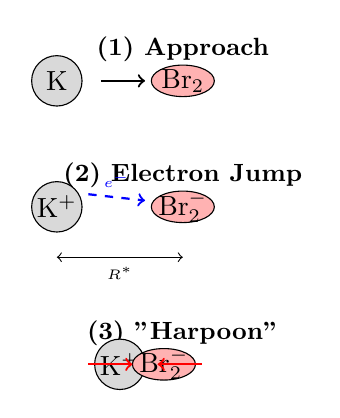
\begin{tikzpicture}[scale=0.8]
% Initial state
\node at (0,3) {\small \textbf{(1) Approach}};
\draw[fill=gray!30] (-2,2.5) circle (0.4cm) node {K};
\draw[fill=red!30] (0,2.5) ellipse (0.5cm and 0.25cm) node {Br$_2$};
\draw[->, thick] (-1.3,2.5) -- (-0.6,2.5);

% Electron transfer
\node at (0,1) {\small \textbf{(2) Electron Jump}};
\draw[fill=gray!30] (-2,0.5) circle (0.4cm) node {K$^+$};
\draw[fill=red!30] (0,0.5) ellipse (0.5cm and 0.25cm) node {Br$_2^-$};
\draw[->, dashed, thick, blue] (-1.5,0.7) -- (-0.6,0.6) node[midway, above] {\tiny $e^-$};
\draw[<->] (-2,-0.3) -- (0,-0.3) node[midway, below] {\tiny $R^*$};

% Attraction
\node at (0,-1.5) {\small \textbf{(3) "Harpoon"}};
\draw[fill=gray!30] (-1,-2) circle (0.4cm) node {K$^+$};
\draw[fill=red!30] (-0.3,-2) ellipse (0.5cm and 0.25cm) node {Br$_2^-$};
\draw[->, thick, red] (-1.5,-2) -- (-0.8,-2);
\draw[->, thick, red] (0.3,-2) -- (-0.4,-2);
\end{tikzpicture}
\end{columns}

\end{frame}

% ===========================================================================
% Slide: Temperature Dependence
% ===========================================================================
\begin{frame}{Temperature Dependence of Reaction Rates}

From collision theory: $k = A T^{1/2} e^{-E_a/RT}$

\vspace{0.2cm}

\textbf{Taking logarithm:}
\[ \ln k = \ln A + \frac{1}{2}\ln T - \frac{E_a}{RT} \]

\textbf{Arrhenius plot} ($\ln k$ vs $1/T$) assumes $A$ is constant:
\[ \ln k = \ln A - \frac{E_a}{RT} \]

\begin{columns}[T]
\column{0.5\textwidth}
\textbf{In practice:}
\begin{itemize}
\item The $T^{1/2}$ factor is weak
\item Over typical experimental ranges (50-100 K), the exponential dominates
\item Arrhenius plots are nearly linear
\item Slope gives $E_a/R$
\end{itemize}

\column{0.5\textwidth}
\centering
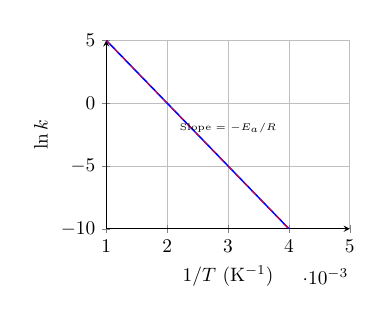
\begin{tikzpicture}[scale=0.7]
\begin{axis}[
    xlabel={$1/T$ (K$^{-1}$)},
    ylabel={$\ln k$},
    axis lines=left,
    grid=major,
    width=6cm,
    height=5cm,
    xmin=0.001, xmax=0.005,
    ymin=-10, ymax=5
]
% Correct Arrhenius plot: ln k decreases as 1/T increases (T decreases)
\addplot[blue, thick, domain=0.001:0.005, samples=50] {10 - 5000*x};
\draw[dashed, red] (axis cs:0.001,5) -- (axis cs:0.005,-15);
\node at (axis cs:0.003,-2) {\tiny Slope = $-E_a/R$};
\end{axis}
\end{tikzpicture}
\end{columns}

\end{frame}

% ===========================================================================
% Slide: Unimolecular Reactions - The Lindemann Mechanism
% ===========================================================================
\begin{frame}{Unimolecular Reactions: The Lindemann Mechanism}

\textbf{Problem:} How can A $\to$ P be explained by collision theory?

\textbf{Lindemann-Hinshelwood Mechanism (1922):}

\begin{enumerate}
\item \textbf{Activation:} A + M $\xrightarrow{k_a}$ A$^*$ + M
\item \textbf{Deactivation:} A$^*$ + M $\xrightarrow{k_a'}$ A + M
\item \textbf{Reaction:} A$^*$ $\xrightarrow{k_b}$ P
\end{enumerate}

\vspace{0.15cm}

\textbf{Key Idea:}
\begin{itemize}
\item A$^*$ = high-energy form of A
\item M = any collision partner
\item Competition: deactivation vs. reaction
\end{itemize}

\emphbox{Two limiting regimes: high pressure and low pressure}

\end{frame}

% ===========================================================================
% Slide: Lindemann Mechanism - Rate Law
% ===========================================================================
\begin{frame}{Lindemann Mechanism: Deriving the Rate Law}

\textbf{Mechanism:}
\begin{align*}
\text{A} + \text{M} &\underset{k_a'}{\overset{k_a}{\rightleftharpoons}} \text{A}^* + \text{M} \\
\text{A}^* &\xrightarrow{k_b} \text{P}
\end{align*}

\textbf{Rate of product formation:} $\frac{d[\text{P}]}{dt} = k_b[\text{A}^*]$

\textbf{Steady-state approximation for A$^*$:}
\[ \frac{d[\text{A}^*]}{dt} = k_a[\text{A}][\text{M}] - k_a'[\text{A}^*][\text{M}] - k_b[\text{A}^*] = 0 \]

\textbf{Solve for [A$^*$]:}
\[ [\text{A}^*] = \frac{k_a[\text{A}][\text{M}]}{k_a'[\text{M}] + k_b} \]

\textbf{Overall rate:}
\keyeq{\frac{d[\text{P}]}{dt} = \frac{k_a k_b [\text{M}]}{k_a'[\text{M}] + k_b} [\text{A}]}

\end{frame}

% ===========================================================================
% Slide: Lindemann - High Pressure Limit
% ===========================================================================
\begin{frame}{Lindemann Mechanism: High Pressure Limit}

\textbf{General Rate Law:}
\[ \frac{d[\text{P}]}{dt} = \frac{k_a k_b [\text{M}]}{k_a'[\text{M}] + k_b} [\text{A}] = k_{uni}[\text{A}] \]

\vspace{0.2cm}

\textbf{High Pressure Limit:} $k_a'[\text{M}] \gg k_b$ (fast deactivation)

\[ k_{uni} \approx \frac{k_a k_b}{k_a'} = K_{eq} k_b \]

\vspace{0.15cm}

\textbf{Characteristics:}
\begin{itemize}
\item First-order in [A]
\item Independent of pressure
\item Rate-determining step: A$^* \to$ P
\item Equilibrium established between A and A$^*$
\item Collisions are frequent enough to maintain equilibrium
\end{itemize}

\end{frame}

% ===========================================================================
% Slide: Lindemann - Low Pressure Limit
% ===========================================================================
\begin{frame}{Lindemann Mechanism: Low Pressure Limit}

\textbf{General Rate Law:}
\[ k_{uni} = \frac{k_a k_b [\text{M}]}{k_a'[\text{M}] + k_b} \]

\vspace{0.4cm}

\textbf{Low Pressure Limit:} $k_a'[\text{M}] \ll k_b$ (slow activation)

\[ k_{uni} \approx k_a[\text{M}] \]

\vspace{0.3cm}

\textbf{Characteristics:}
\begin{itemize}
\item Pseudo-second-order (depends on [M])
\item Proportional to pressure
\item Rate-determining step: A + M $\to$ A$^*$
\item Every A$^*$ formed reacts immediately ($k_b$ is fast)
\item Collisions are rare, activation is limiting
\end{itemize}

\vspace{0.3cm}

\emphbox{Transition from second-order to first-order as pressure increases}

\end{frame}

% ===========================================================================
% Slide: Lindemann Plot
% ===========================================================================
\begin{frame}{Lindemann Mechanism: Graphical Representation}

\textbf{Rearrange to Lindemann form:}
\[ \frac{1}{k_{uni}} = \frac{1}{k_\infty} + \frac{k_a'}{k_a k_b[\text{M}]} = \frac{1}{k_\infty} + \frac{1}{k_a[\text{M}]} \]

where $k_\infty = \frac{k_a k_b}{k_a'}$ is the high-pressure limit.

\begin{columns}[T]
\column{0.5\textwidth}
\textbf{Lindemann Plot:}
$1/k_{uni}$ vs $1/[\text{M}]$
\begin{itemize}
\item Linear relationship
\item Intercept = $1/k_\infty$
\item Slope = $1/k_a$
\end{itemize}

\column{0.5\textwidth}
\centering
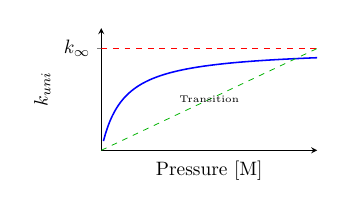
\begin{tikzpicture}[scale=0.7]
\begin{axis}[
    xlabel={Pressure [M]},
    ylabel={$k_{uni}$},
    axis lines=left,
    xmin=0, xmax=10,
    ymin=0, ymax=6,
    xtick=\empty,
    ytick={5},
    yticklabels={$k_\infty$},
    width=5.5cm,
    height=3.8cm
]
\addplot[blue, thick, domain=0.1:10, samples=100] {5*x/(x+1)};
\draw[dashed, red] (axis cs:0,5) -- (axis cs:10,5) node[right] {\tiny First-order};
\draw[dashed, green!70!black] (axis cs:0,0) -- (axis cs:10,5) node[below right] {\tiny Second-order};
\node at (axis cs:5,2.5) {\tiny Transition};
\end{axis}
\end{tikzpicture}
\end{columns}

\vspace{0.1cm}

{\small \textbf{Experimental verification:} Many unimolecular reactions show exactly this behavior!}

\end{frame}

% ===========================================================================
% Slide: RRK Theory - Part 1
% ===========================================================================
\begin{frame}{RRK Theory: Energy Distribution in Molecules (Part 1)}

\textbf{Rice-Ramsperger-Kassel (RRK) Theory:}

Refines Lindemann by considering \textit{how} energy is distributed within A$^*$.

\vspace{0.3cm}

\textbf{Key Assumptions:}
\begin{itemize}
\item Molecule has $s$ equivalent oscillators (vibrational modes)
\item Energy $E$ is distributed randomly among these modes (statistical)
\item Reaction occurs when energy $E_0$ accumulates in the reactive bond
\item Energy flows freely between modes (ergodic hypothesis)
\end{itemize}

\vspace{0.3cm}

\textbf{Key Question:} What is the probability that the reactive bond has enough energy to break?

\end{frame}

% ===========================================================================
% Slide: RRK Theory - Part 2
% ===========================================================================
\begin{frame}{RRK Theory: Energy-Dependent Rate Constant (Part 2)}

\textbf{Probability that reactive bond has energy $\ge E_0$:}
\[ P(E_0|E) = \left(1 - \frac{E_0}{E}\right)^{s-1} \quad \text{for } E \ge E_0 \]

\vspace{0.3cm}

\textbf{Energy-dependent rate constant:}
\keyeq{k_b(E) = k_b^0 \left(1 - \frac{E_0}{E}\right)^{s-1}}

\vspace{0.3cm}

\textbf{Physical Interpretation:}
\begin{itemize}
\item Higher $s$ (more oscillators): Energy more diluted, slower reaction
\item Larger molecules: Smaller $k_b(E)$ at given $E$
\item Explains why large molecules fall off more rapidly in Lindemann plots
\end{itemize}

\end{frame}

% ===========================================================================
% Slide: Summary of Collision Theory
% ===========================================================================
\begin{frame}{Summary: Collision Theory}

\textbf{Achievements:}
\begin{itemize}
\item[\checkmark] Derived rate constant from first principles (kinetic theory)
\item[\checkmark] Explained Arrhenius form: $k = A e^{-E_a/RT}$
\item[\checkmark] Calculated $A$-factors ($\sim 10^{10}-10^{11}$ dm$^3$ mol$^{-1}$ s$^{-1}$)
\item[\checkmark] Lindemann mechanism explains unimolecular reactions
\item[\checkmark] Qualitative understanding of steric effects
\end{itemize}

\vspace{0.3cm}

\textbf{Limitations:}
\begin{itemize}
\item[\xmark] Steric factor $P$ is empirical (must be measured)
\item[\xmark] Hard-sphere model too simplistic
\item[\xmark] Doesn't explain molecular details of reaction pathway
\item[\xmark] No information about transition state structure
\end{itemize}

\vspace{0.3cm}

\emphbox{Next: Transition-State Theory provides molecular-level insight}

\end{frame}

% ===========================================================================
% Slide: Practice Problems
% ===========================================================================
\begin{frame}{Practice Problems}

\textbf{Problem 1:} Calculate the collision frequency $Z_{O_2-O_2}$ for oxygen at 300 K and 1 atm. Use $\sigma = 0.40$ nm$^2$.

\vspace{0.2cm}

\textbf{Problem 2:} For the reaction H$_2$ + I$_2 \to$ 2HI, $E_a = 171$ kJ mol$^{-1}$. What fraction of collisions at 600 K have sufficient energy to react?

\vspace{0.2cm}

\textbf{Problem 3:} A reaction has $A_{exp} = 2.5 \times 10^{9}$ dm$^3$ mol$^{-1}$ s$^{-1}$ and $A_{theory} = 5.0 \times 10^{11}$ dm$^3$ mol$^{-1}$ s$^{-1}$. Calculate the steric factor $P$. What does this tell you about the reaction?

\vspace{0.2cm}

\textbf{Problem 4:} For a Lindemann mechanism with $k_\infty = 1.0 \times 10^5$ s$^{-1}$ and $k_a = 1.0 \times 10^{-10}$ dm$^3$ mol$^{-1}$ s$^{-1}$, at what pressure (in torr) does $k_{uni} = k_\infty/2$? (T = 300 K)

\vspace{0.2cm}

\textit{Answers: (1) $\sim 10^{35}$ m$^{-3}$ s$^{-1}$; (2) $e^{-171000/(8.314 \times 600)} \approx 1.7 \times 10^{-15}$; (3) $P = 0.005$, highly orientation-dependent; (4) $\sim 0.04$ torr}

\end{frame}

% ===========================================================================
% Slide: Interactive Resources for Topic 18A
% ===========================================================================
\begin{frame}{Interactive Learning: Topic 18A}

\begin{columns}[c]
\column{0.65\textwidth}
\textbf{Explore Collision Theory Interactively!}

\vspace{0.3cm}

\textbf{Interactive Jupyter Notebook Features:}
\begin{itemize}
    \item \textbf{Collision Calculator}: Adjust T, P, $\sigma$ with sliders
    \item \textbf{Animated Collisions}: Watch molecules collide!
    \item \textbf{Energy-Dependent $\sigma(\varepsilon)$}: Interactive plots
    \item \textbf{Harpoon Mechanism Explorer}: See long-range ET
    \item \textbf{RRK Model}: Explore unimolecular decay
    \item \textbf{Practice Problems}: Code-based exercises
\end{itemize}

\vspace{0.3cm}

\textbf{Notebook:} \texttt{01\_Collision\_Theory.ipynb}

\column{0.35\textwidth}
\centering
\textbf{Scan to Open:}

\vspace{0.3cm}

\includegraphics[width=0.8\textwidth]{QR_codes/01_Collision_Theory.png}

\vspace{0.3cm}

{\footnotesize Or navigate to:\\
\texttt{Reaction\_Dynamics\_Interactive/}}

\end{columns}

\end{frame}
